% 下面我大概想了一下分点, 如果觉得有更好表达方法可以合并/拆分这些section自由发挥
\section{功能模块说明}
从功能设计的角度, 我们的工具按执行顺序主要分为自动化测试执行、自动化测试结果分析、复现引导。

\subsection{自动化测试执行}
在自动化测试执行阶段,我们共做了两种尝试。
首先在Appium框架的基础上应用monkey工具对目标安卓应用进行随机测试,通过调整随机动作的比例和间隔尝试触发bug,将成功触发bug的log保存为文件,每个动作的参数包括动作类型(按下、抬起、翻转、截图等)和作用坐标。

由于monkey工具不支持在运行的同时保存每次动作前后的截图状态,我们额外使用/test/script中代码自定义动作复现被monkey触发的bug,以获取行动链每个节点的截图。自动化测试执行的结果再经过下一步“测试结果分析”处理,以备引导复现使用。

\subsection{自动化测试结果分析}
每次monkey运行发现一个bug,都会将发现错误的过程截图保存到一个文件夹下,但是monkey在运行过程中是随机操作的,因此会生成一个非常冗长的操作序列,我们很难确定最终的bug是由哪些序列引起的,在项目中,我们采用了一些简单的手段进行处理。
\begin{itemize}
    \item 邻近图片去重:monkey可能会随意点击而无法触发任何交互效果,我们使用图片相似度分析的手段寻找相邻且高度相似的图片,仅保留一张
    \item 寻找开始与结束序列:无论monkey如何执行序列,开始序列的第一张图应当是手机的Home界面,我们将Home界面作为一段执行序列入口,找到两个邻近并且包含了引发crash的操作截图的入口,仅保留这两个入口间的截图即可
    \item 我们没有设计将特定组件识别并且展示给用户的功能,为了方便用户交互,我们围绕monkey给出的location参数以一定的半径画一个圈,以此来提示用户点击、滑动等操作
\end{itemize}

但是经过这些处理后的效果仍然不理想,最后我们还是对bug图像序列进行了一些手动修正。



\subsection{复现引导}
\subsubsection{对话系统的实现}
% @wct
我们设计了一个轻量的对话系统. 具体来说, 后端使用 \lstinline{Python Flask} 框架, 前端使用纯 \lstinline{html} 与 \lstinline{css} 实现. 我们选取了 \lstinline{Python SpaCy} 库中的 \lstinline{en_core_web_sm} 小型语言模型用作自然语言处理. 

我们考虑到当前的场景是高度专业化的, 因此对话系统的功能设计也是针对性的. 出于这样的想法, 我们并没有接入更大的语言模型, 而是在本地规定了一些常见的问题作为语料库, 使用 \lstinline{SpaCy} 库的 \lstinline{similarity()} 函数作为相似度的度量. 基本的想法是, 如果用户提出了一个问题, 那么我们就在语料库中寻找与之相似的问题, 并返回相应的答案. 对应的代码如下:
\scalebox{0.96}{
    \lstinputlisting[language=Python]{gist/nlp.txt}
}

在实现的过程中, 我们主要将用户的问题分成了如下的几类, 并给出相应的回答:
\begin{itemize}
    \item \lstinline{[ERROR]}: ``I'm sorry, I can't understand you.''
    \item \lstinline{[GREETING]}: ``Hello, what can I help you?''
    \item \lstinline{[NEXT]}: ``You are supposed to reach this step as shown in the following screenshot.''
    \item \lstinline{[CURRENT-STATE]}: ``Your current step is as follows.''
    \item \lstinline{[HELP]}: ``I am REP-FLOW, and I have a certain level of conversational ability. You can ask me the following questions..''
    \item \lstinline{[SORRY]}: ``I'm sorry, I'm a simple chatbot, which means that I can only help you reproduce the bug according to the recorded steps. If you want to reproduce the bug in other ways, please try again.''
    \item \lstinline{[TEST]}: ``Sure thing! You can try reproducing the bug yourself, and I would monitor your actions and record the steps. If you are not sure what the next step is at a certain point, you can ask me. e.g. 'What's the next Step?''
    \item \lstinline{[ID-MISSING]}: ``Please tell me the bug number first, e.g. /test 114514.''
    \item etc.
\end{itemize}

这样的设计使得我们的对话系统即满足领域专业化的要求, 又能够在一定程度上满足用户的需求. 例如, 如果用户在复现的过程中不知道下一步是什么, 那么他可以根据指示点击 \lstinline{/next} 指令 (如图\ref{fig:cmd}), 也可以直接问对话系统下一步是什么 (如图\ref{fig:chat}).

\begin{figure}[H]
    \centering
    \begin{subfigure}{0.45\textwidth}{
        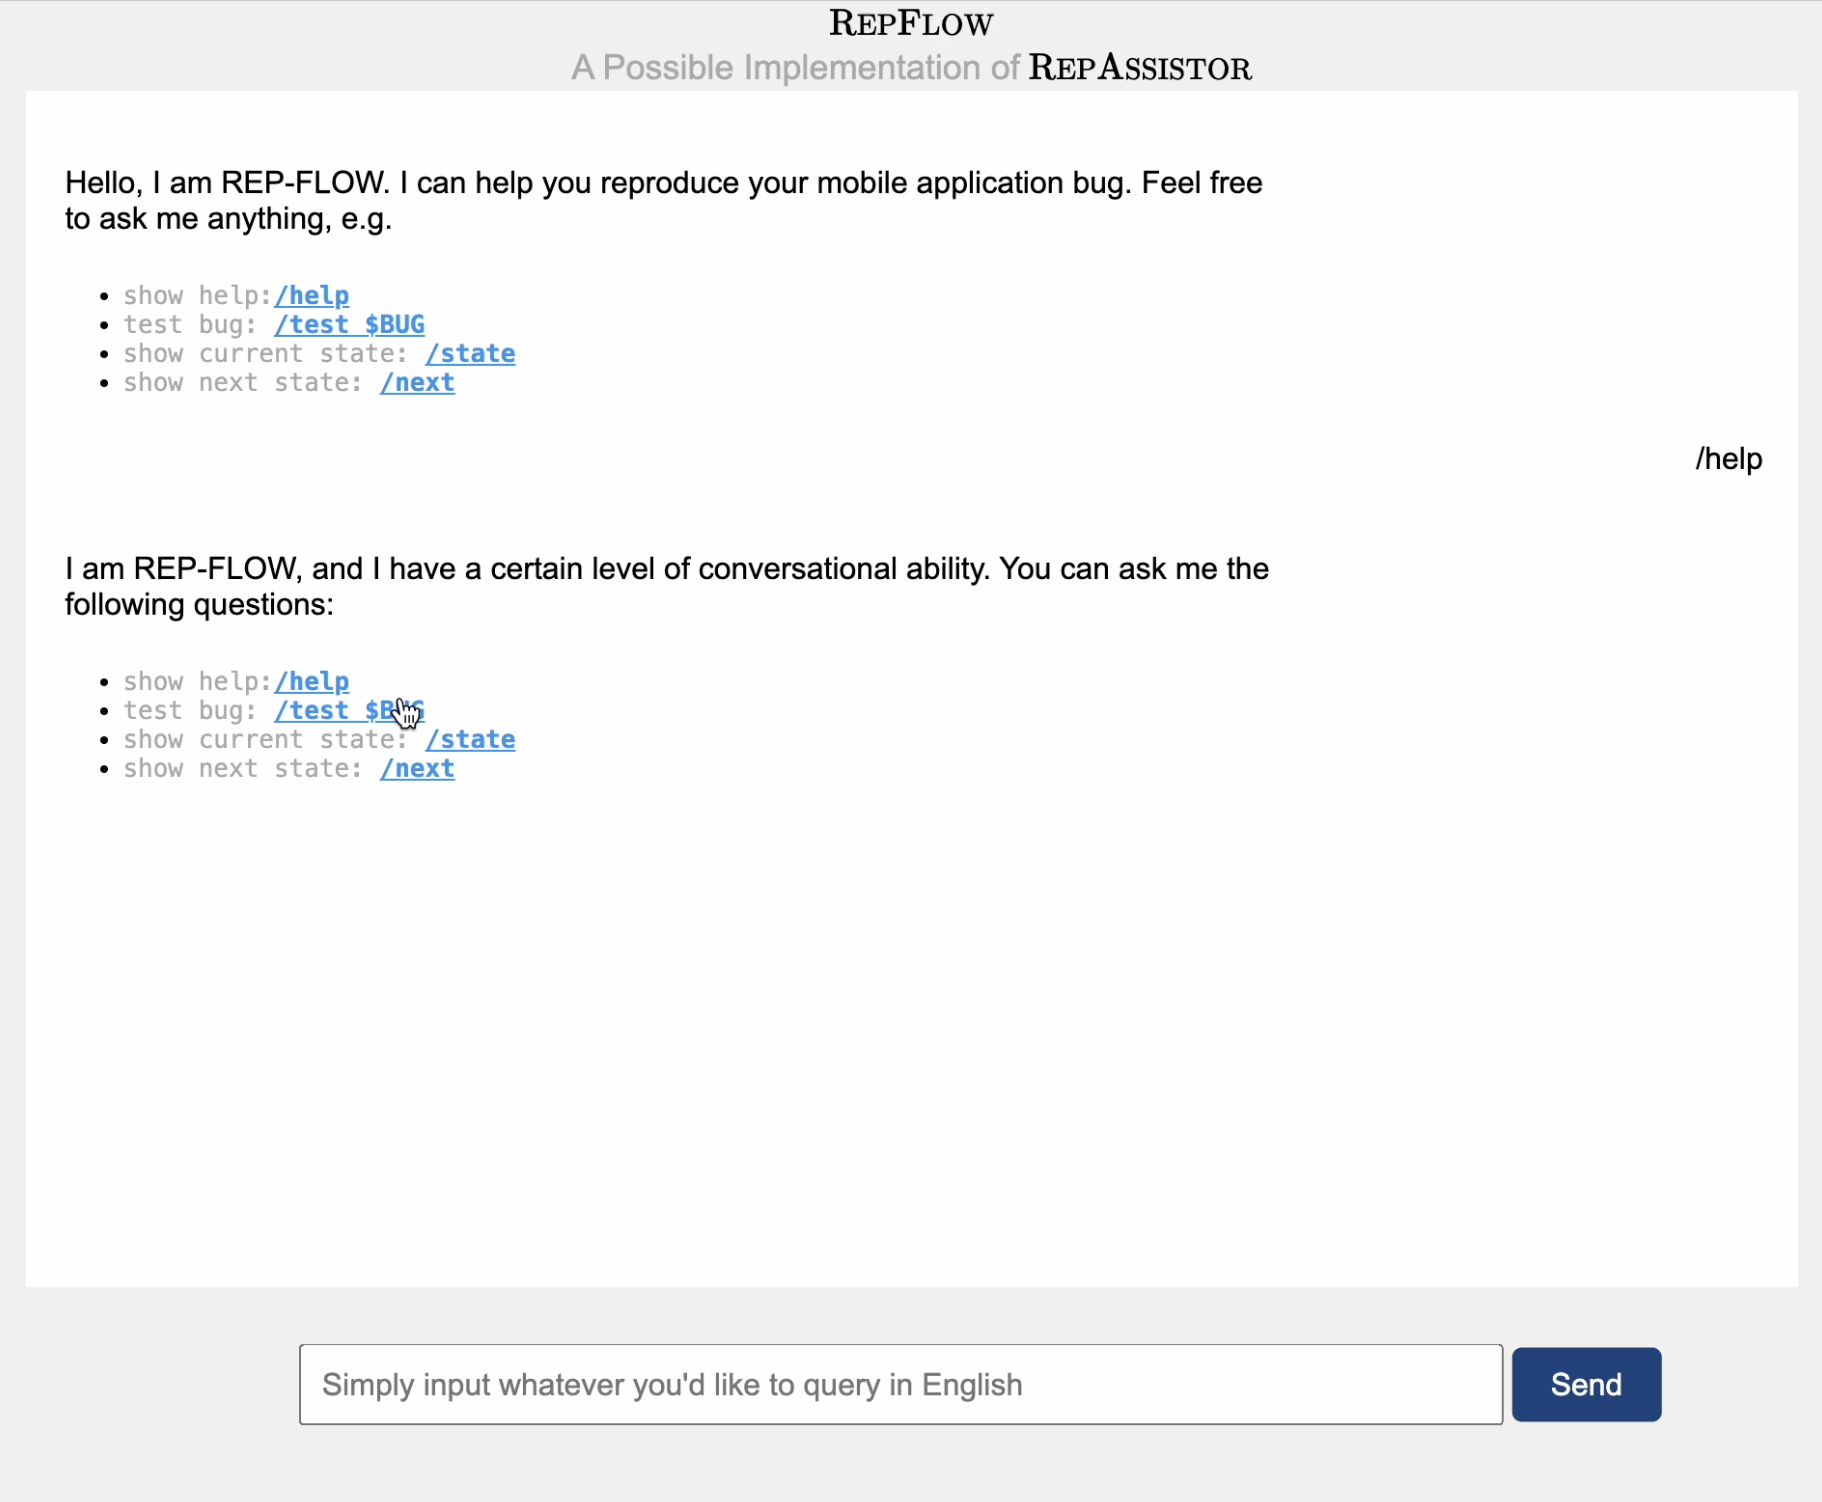
\includegraphics[width=\linewidth]{figures/cmd.png}
        \caption{[对话系统]提示}\label{fig:cmd}
    }
    \end{subfigure}
    \begin{subfigure}{0.465\textwidth}{
        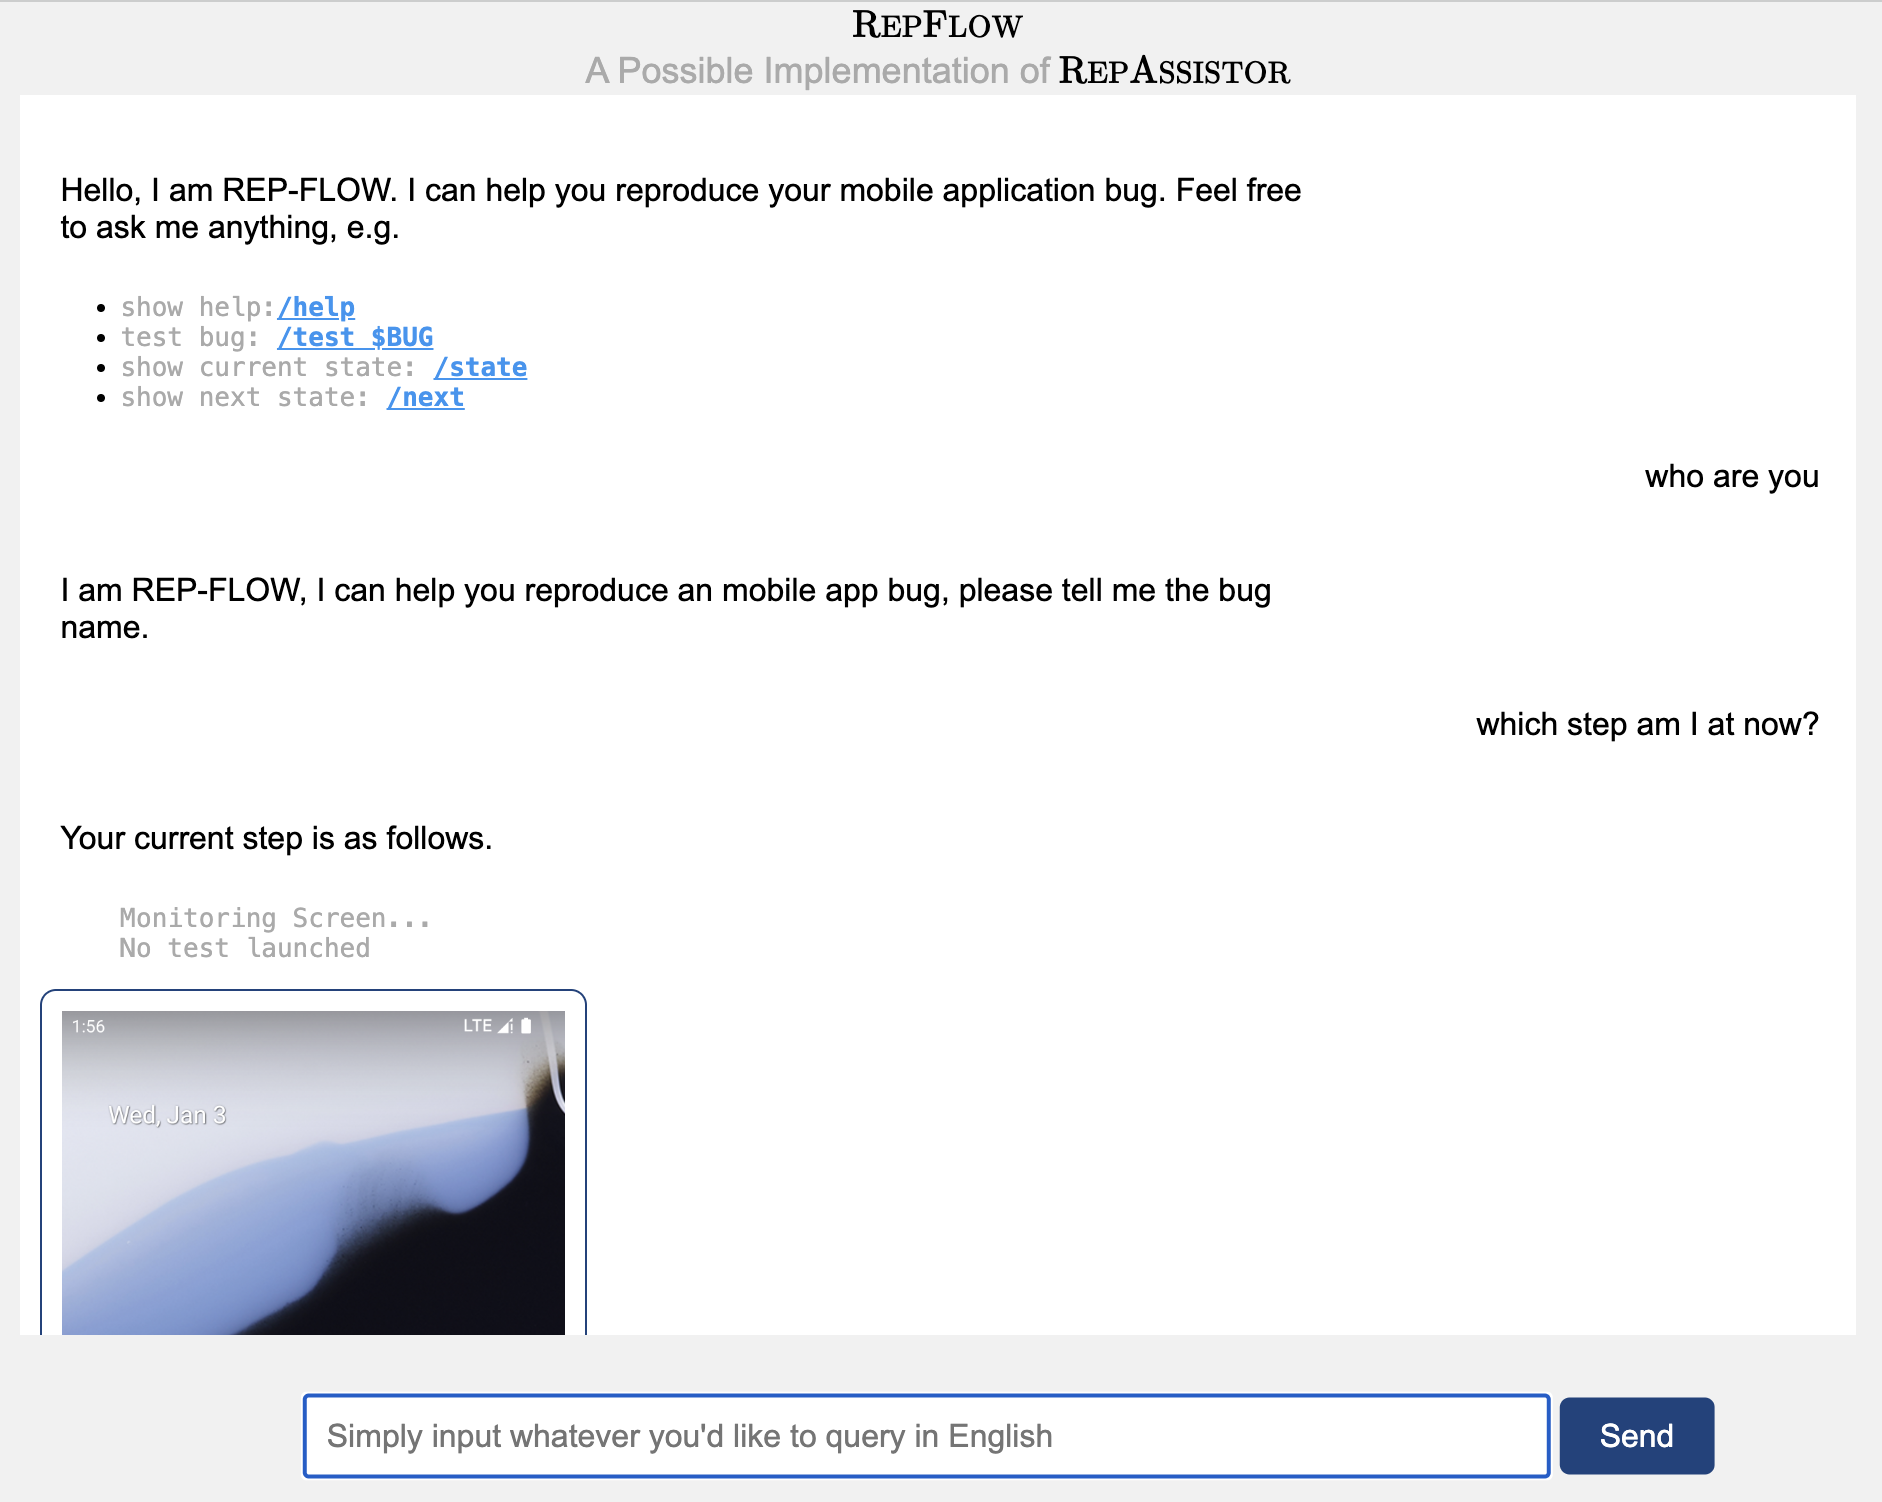
\includegraphics[width=\linewidth]{figures/chat.png}
        \caption{[对话系统]对话}\label{fig:chat}
    }
    \end{subfigure}
\end{figure}



\subsubsection{状态提取}
% @wct
我们使用 \lstinline{Appium} 来获取用户屏幕的状态. 当对话系统启动时, 启动个新的进程来运行 \lstinline{Appium} 脚本. 我们规定, 如果:
\begin{enumerate}
    \item 当前页面的 \lstinline{xml} 结构和上一个时刻的 \lstinline{xml} 结构不同, 那么就认为用户进行了一次操作; 或者
    \item 当前页面的任何一个 \lstinline{Button} 元素被点击 (通过 XPath 来实现); 或者
    \item 当前页面还没有被截图过.
\end{enumerate}
那么就截取图片并且存储在本地, 当前端请求的时候发送给前端. 具体来说, 我们使用如下的 \lstinline{while} 循环来实现:

\scalebox{0.9}{
    \lstinputlisting[language=Python]{gist/state.txt}
}
\subsubsection{图片相似度分析}

为了确认用户在bug的复现流程中处于哪一步, 我们需要对当前用户截屏和bug复现截屏流进行图片相似度分析, 因此我们使用了以下两种相似度分析算法模型.
\begin{enumerate}
    \item 三直方图算法模型. 算法主要基于图像的颜色信息,通过比较图像的颜色直方图来评估它们之间的相似性. 代码如下:
    
    \scalebox{0.9}{
        \lstinputlisting[language=Python]{gist/hist.txt}
    }
    \item 结构相似性算法模型. 算法主要通过分别比较两个图像的亮度,对比度,结构,然后对这三个要素加权并用乘积表示. 代码如下:

    \scalebox{0.9}{
        \lstinputlisting[language=Python]{gist/ssim.txt}
    }
\end{enumerate}

为了提升图片相似度分析的准确率, 我们采取加权平均的方式综合两种算法模型的结果, 当最大综合相似度>0.65时认为找到了用户所处的bug复现位置, 反之则认为用户脱离了正常的bug复现流程. 具体实现代码如下:

\scalebox{0.9}{
    \lstinputlisting[language=Python]{gist/process.txt}
}

我们注意到, 结构相似性算法模型的时间开销明显大于三直方图算法模型, 所以提供了另一个只使用三直方图算法模型的函数接口, 该函数的运行速度是上一种函数的十倍左右。当最大相似度>0.7时认为找到了用户所处的bug复现位置, 反之则认为用户脱离了正常的bug复现流程.

当在对图片相似度分析的准确度要求不高的情况下, 我们选择第二种函数, 以提高对话系统的整体反应速度. 具体实现代码如下:

\scalebox{0.9}{
    \lstinputlisting[language=Python]{gist/process_faster.txt}
}